\section{Ejercicios}

\subsection{Ejercicio 1: TaskConsola}
En \'este ejercicio debemos programar una tarea \textit{TaskConsola} la cual debe realizar n llamadas bloqueantes, cada una con 
una duraci\'on al azar entre bmin y bmax, ambas pasadas por par\'ametro.

Para ello, decidimos utilizar un contador de 0 hasta n y generar un n\'umero pseudo-alaeatorio por medio de la 
funci\'on \textit{rand}. Es decir, cada vez que se aumenta el contador, realizamos una llamada bloqueante (uso\_IO) 
que durar\'a la cantidad de ciclos que se haya generado en la llamada a rand.

\subsection{Ejercicio 2: Experimentando FCFS}
Para probar el Scheduler First Came First Served usaremos el siguiente lote de tareas:

\begin{center}
TaskCPU 10\\
TaskConsola 5 1 5\\
TaskConsola 3 1 2
\end{center}

En la primera, utlizaremos TaskCPU y para darle uso intensivo correr\'a durante 10 ciclos de reloj.
Las siguientes, son de tipo TaskConsola implementado anteriormente, pas\'andole como par\'ametro el n\'umero de llamadas 
bloqueantes y el rango en el cual debe seleccionar el n\'umero aleatorio.

En el algoritmo FCFS, la CPU se asigna a los procesos en el orden en que la solicitan.\\
Por lo tanto, esperamos observar que, con un solo n\'ucleo, un proceso no pueda correr 
hasta que no terminaron los anteriores a el.

Con dos nucleos, correr\'an dos procesos simlt\'aneamente y el \'ultimo empezar\'a cuando alguno de los otros dos finalicen,
y por \'ultimo, si el procesador tiene 3 n\'ucleos, los 3 correr\'an al mismo tiempo.

\vspace{\baselineskip}
\begin{center}
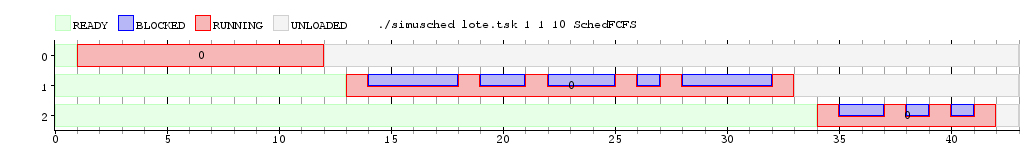
\includegraphics[scale=0.45]{../tp1/Test/resEj2Co1.png}
\\
\vspace{1pt}
\footnotesize\textit{Simulacro FCFS con un n\'ucleo}
\end{center}
\vspace{\baselineskip}


\vspace{\baselineskip}
\begin{center}
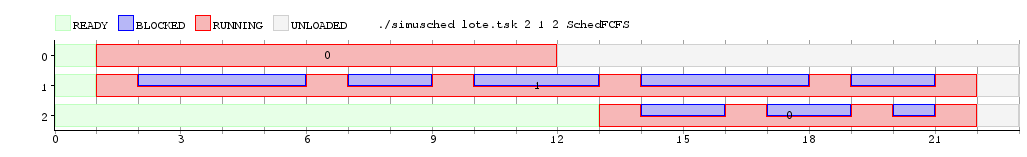
\includegraphics[scale=0.45]{../tp1/Test/resEj2Co2.png}
\\
\vspace{1pt}
\footnotesize\textit{Simulacro FCFS con dos n\'ucleos}
\end{center}
\vspace{\baselineskip}

\vspace{\baselineskip}
\begin{center}
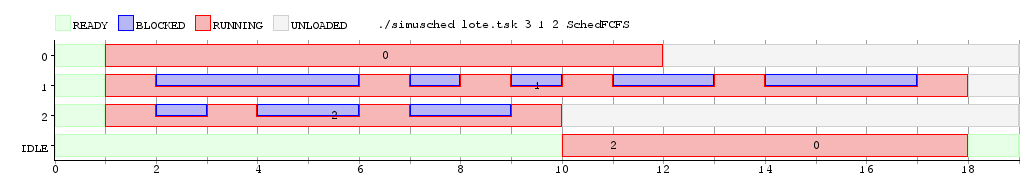
\includegraphics[scale=0.45]{../tp1/Test/resEj2Co3.png}
\\
\vspace{1pt}
\footnotesize\textit{Simulacro FCFS con tres n\'ucleos}
\end{center}
\vspace{\baselineskip}


Como podemos observar, los experimentos resultaron satisfactoriamente con nuestra hip\'otesis.

Adem\'as, notemos que en los casos en los que utilizamos la tarea TaskConsola, se observan claramente
las llamadas bloqueantes de manera random, dado que el tiempo tanto de la ejecuci\'on como el de las llamadas bloqueantes var\'ia.
En el caso en que el procesador tiene tres n\'ucleos, se observa que los n\'ucleos 2 y 0 ejecutan 
Idle ya que est\'an desocupadas, esperando la solicitud del pr\'oximo proceso.

\subsection{Ejercicio 3: Implementando Round-Robin}
La idea del scheduler \textit{Round-Robin} es darle un quantum a cada procesador, cuando un proceso lo solicita,
si alg\'un n\'ucleo esta desocupado, corre la tarea el tiempo que sea el quantum del procesador seleccionado.

Con esta idea desarrollamos nuestro Scheduler Round-Robin. Utilizamos como estructura una Cola $(q)$, para las llamadas a los procesos, 
un vector $(quantum)$ de tama\~no cantidad de cores del procesador que asignar\'a el quantum del i\'esimo n\'ucleo, 
y otro vector $(contador)$ que va a llevar cuenta del tiempo corrido por el proceso en el i\'esimo n\'ucleo hasta llegar al quantum del mismo.

Para el correcto funcionamiento en la funci\'on $tick$ se ven reflejados los casos en el cual el proceso debe 
dejar de correr ya sea porque termin\'o su tiempo o el quantum del procesador en el que corr\'ia. En \'este \'ultimo 
caso, la posici\'on correspondiente al n\'ucleo en $contador$ volver\'a a cero y el proceso se encolar\'a para terminar con su tiempo. 
\\Una vez realizada dicha acci\'on, debe dar lugar a la siguiente en la cola, o en caso de no haber una la Idle 
deber\'a hacerlo hasta el llamado de una nueva.

\subsection{Ejercicio 4: Experimentando Round-Robin}

En este ejercicio nos proponemos experimentar con el scheduler del punto anterior para verificar que el comportamiento es el esperado. Haremos esto de 
manera incremental, es decir, empezaremos probando las cosas mas basicas e iremos subiendo la complejidad. 

Para empezar, probaremos RR con un solo nucleo. Notese que si le asignamos una sola tarea, su comportamiento no diferiria de algun otro scheduler, por
lo que empezamos probando con cuatro tareas simultaneas. Estas tareas solo usan al cpu, por lo tanto no se bloquean. Esperamos 
verificar que el scheduler RR le asigna el tiempo del quantum a cada tarea antes de comenzar de nuevo la lista de tareas pendientes.

\vspace{\baselineskip}
\begin{center}
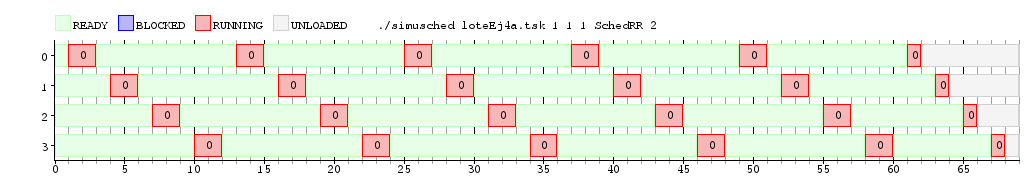
\includegraphics[scale=0.45]{../tp1/Test/resEj4Co1SB.png}
\\
\vspace{1pt}
\footnotesize\textit{Simulacro RR con un n\'ucleo}
\end{center}
\vspace{\baselineskip}

Efectivamente, cuando recibe k tareas simultaneas, el scheduler le asigna tiempo de ejecucion a las tareas de modo que todas 
ejecuten antes de regresar a ejecutar la primera. 

A continuacion usaremos el mismo lote de tareas, pero agregaremos otro procesador. Asi veremos si el scheduler maneja correctamente 
los procesadores para asegurarse que todas las tareas ejecuten un tiempo $quantum$ antes de volver a empezar.

\vspace{\baselineskip}
\begin{center}
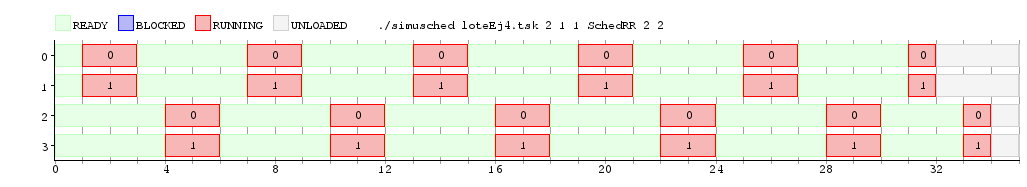
\includegraphics[scale=0.45]{../tp1/Test/resEj4Co2SB.png}
\\
\vspace{1pt}
\footnotesize\textit{Simulacro RR con dos n\'ucleo}
\end{center}
\vspace{\baselineskip}

El comportamiento es identico al anterior, solo que agregando otro nucleo, es decir, podemos deducir las mismas concluciones. Para probar de 
modo mas realista este scheduler, vamos a simular un lote de cuatro tareas que realicen llamadas bloqueantes, con dos procesadores para su ejecucion.
Lo que queremos mostrar, es que el scheduler trabajara de manera optima en este caso.

\vspace{\baselineskip}
\begin{center}
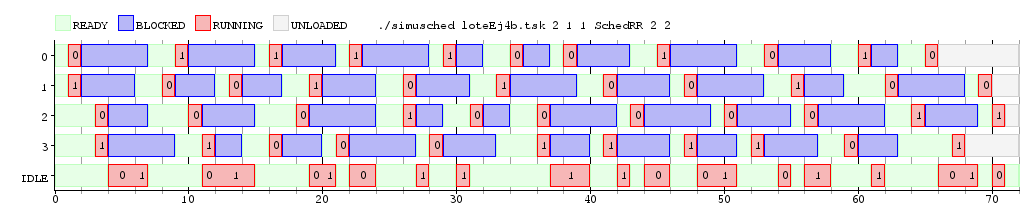
\includegraphics[scale=0.45]{../tp1/Test/resEj4Co2CB.png}
\\
\vspace{1pt}
\footnotesize\textit{Simulacro RR con dos n\'ucleo}
\end{center}
\vspace{\baselineskip}

Podemos ver que el scheduler trabaja de la manera esperada. Es decir, si hay un tarea disponible para ejecutar y procesador que no esta ejecutando nada,
ese procesador carga la tarea y la ejecuta, o bien hasta que se le acabe el quantum o hasta que se bloquee. Si todas las tareas estan bloqueadas 
o ejecutando cuando el procesador termina la ejecucion de una tarea porque se bloqueo, este se poner a ejecutar la tarea IDLE hasta que 
una tarea se desbloque. Y por lo tanto, si todas las tareas estan bloqueadas, ambos procesadores ejecutan la tarea IDLE hasta que alguna 
tarea se desbloquee.



\subsection{Ejercicio 5}
\subsection{Ejercicio 6: TaskBatch}

En este ejercicio implementamos la tarea TaskBatch, que recibe como parametros totalcpu y cantbloqueos. Esta tarea dura totalcpu tiempo de 
cpu, y realiza cantbloqueos llamadas bloqueantes en momentos psudoaleatorios. Realizamos de dos maneras. La primera implementacion toma iteraba totalcpu
veces pidiendo un numero aleatorio rand. Si rand > 0.5 entonces llama a una tarea bloqueante, sino, a una tarea que use el cpu. Si la cantidad 
de iteraciones se acaba sin haber realizado todas las llamadas bloqueantes, entonces se realizaban las restantes seguidas al final. Sino, cuando se realizaba
la ultima llamada bloqueante, se utilizaba el tiempo restante del cpu todo junto. Lo que observamos en esta implementacion fue que las llamadas bloqueantes
se hacian para tiempos grandes siempre al principio del intervalo de uso del cpu, y para tiempos de medianos a cortos, siempre al final.**********

Por eso realizamos otra implementacion. En esta se seleccionan previamente en que momentos se van a realizar las llamadas bloqueantes, y luego se itera 
sobre el tiempo del cpu.


\subsection{Ejercicio 7}
\subsection{Ejercicio 8: Round Robin sin migracion}
\subsection{Ejercicio 9}
\subsection{Ejercicio 10}